% Messwerte: Alle gemessenen Größen tabellarisch darstellen
% Auswertung: Berechnung geforderter Ergebnisse mit Schritten/Fehlerformeln/Erläuterung/Grafik (Programme)
\section{Auswertung}
\label{sec:auswertung}
Im Folgenden wird die Kennlinie des Geiger-Müller Zählrohrs bestimmt und 
die Anzahl der Ladungträger wird anhand der Messwerte berechnet. Die Totzeit wird zunächst über die Zwei-Quellen-Methode
und im Anschluss über das Osziloskop bestimmt.

\subsection{Fehlerrechnung}
\label{sec:Fehlerrechnung}
Die Fehlerrechnung, für die Bestimmung der Messunsicherheiten, wird mit Uncertainties \cite{uncertainties} gemacht.
Für die Formel der Gauß Fehlerfortpflanzung ist gegeben durch
\begin{equation}
    \Delta f=\sqrt{\sum_{i=1}^N\left(\frac{\partial f}{\partial x_i}\right)^2 \cdot\left(\Delta x_i\right)^2}.
    \label{eqn:gauss}
\end{equation}
Für den Mittelwert gilt 
\begin{equation}
    \bar{x} = \frac{1}{N}\sum\limits_{i = 1}^N x_i .
    \label{eqn:mittelwert}
\end{equation}
Der Fehler des Mittelwertes ist gegeben durch 
\begin{equation}
    \Delta \bar{x}=\frac{1}{\sqrt{N}} \sqrt{\frac{1}{N-1} \sum_{i=1}^N\left(x_i-\bar{x}\right)^2}.
    \label{eqn:mittelwertfehler}
\end{equation}

\subsection{Kennlinie des Geiger-Müller-Zählrohrs}
\label{sec:Kennlinie des Geiger-Müller-Zählrohrs}

Die aufgenommenen Messwerte zur Bestimmung der Kennlinie des Geiger-Müller-Zählrohrs sind in der \autoref{tab:kennlinie}
dargestellt. Zudem wurde mit Hilfe der \autoref{eqn:} der statistische Fehler $\lambda$ bestimmt und ebenfalls aufgelistet.
Der Plateau-Bereich hat eine Länge von $\SI{340}{\volt}$ , dieser beginnt bei $\SI{370}{\volt}$ und hört bei $\SI{710}{\volt}$ auf.
Im ersten drittel des Plateaus lässt sich der Arbeitspunkt bei $U_A = 430$ ablesen.

\begin{table}[H]
    \centering
    \caption{Messdaten zur Bestimmung der Kennlinie des Geiger-Müller-Zählrohrs}
    \label{tab:kennlinie}
\begin{tabular}{c c c c}
    \toprule
    $U \mathbin{/} \mathrm{V}$ & $N$ &  $I \mathbin{/} \unit{\micro\ampere}$ & $\lambda$\\
    \midrule
         330 &    17211 &   0.2 & 131\\
         350 &    18298 &   0.2 & 135\\
         370 &    18392 &   0.3 & 136\\
         390 &    18818 &   0.4 & 137\\
         410 &    18653 &   0.4 & 137\\
         $\textbf{430}$ &    $\textbf{18946}$ &   $\textbf{0.5}$ & $\textbf{138}$\\
         450 &    18915 &   0.6 & 138\\
         470 &    18905 &   0.7 & 137\\
         490 &    18934 &   0.8 & 138\\
         510 &    18970 &   0.8 & 138\\
         530 &    19015 &   0.8 & 138\\
         550 &    19336 &   0.9 & 139\\
         570 &    19235 &     1 & 139\\
         590 &    19174 &     1 & 138\\
         610 &    19224 &   1.1 & 139\\
         630 &    18991 &   1.2 & 138\\
         650 &    19082 &   1.2 & 138\\
         670 &    19548 &   1.3 & 140\\
         690 &    19505 &   1.3 & 140\\
         710 &    20031 &   1.4 & 142\\
         730 &    20429 &   1.5 & 143\\
         750 &    21666 &   1.6 & 147\\
    \bottomrule
    \end{tabular}
\end{table}


Die Messdaten der Detektorspannung $U$ wurden gegen die Zählrate $N$ aufgetragen und in der
\autoref{fig:plot_1} dargestellt. Die Ausgleichsgrade hat die Form
\begin{equation*}
    N = a \cdot U + b.
\end{equation*}
Die Gerade beschreibt den Plateau-Bereich. Der Parameter $a$ beschreibt die Plateau-Steigung des Geiger-Müller-Zählrohrs.
Mit Hilfe von Linearer Regression, welche mit SciPy \cite{scipy} durchgeführt wurde, ergeben sich die Werte
\begin{align*}
    a &= \qty{0.018(3)}{\per\volt} \quad \text{und} \\
    b &= \num{149.499(1720)} \, .
\end{align*}

\begin{figure}[H]
	\includegraphics{build/plot_1.pdf}
	\caption{Messwerte der Detektorspannung wurde gegen die Zählrate aufgetragen. Zudem die Ausgleichsgrade des Plateu-Bereichs.}
	\label{fig:plot_1}
\end{figure}

\subsection{Anzahl der detektierten Ladungsträger}
\label{sec:Anzahl der detektierten Ladungsträger}

In der \autoref{tab:ladungs} sind die gemessenen Werte für die  Spannung $U$ und die Stromstärke $I$ abgebildet.
Zusätzlich wurde die Anzahl der detektierten Ladungsträger $Z$ pro einfallenden Teilchen anhand der Formel
\begin{equation*}
    Z = \frac{t \cdot I}{e}
\end{equation*}
berechnet. Dabei beträgt $t = \SI{120}{\second}$ und die Elementarladung $e$ ist gegeben durch $e = 1.6 \cdot 10^{-19} \si{coulomb}$.

\begin{table}[H]
    \centering
    \caption{Anzahl der Ladungsträger gegen die Detektorspannung aufgetragen.}
    \label{tab:ladungs}
\begin{tabular}{c c c c}
    \toprule
    $U \mathbin{/} \mathrm{V}$ & $N$ &  $I \mathbin{/} \unit{\micro\ampere}$ & $Z \cdot 10^{14}$\\
    \midrule
         330 &    17211 &   0.2 & 1.498\\
         350 &    18298 &   0.2 & 1.498\\
         370 &    18392 &   0.3 & 2.247\\
         390 &    18818 &   0.4 & 2.996\\
         410 &    18653 &   0.4 & 2.996\\
         430 &    18946 &   0.5 & 3.745\\
         450 &    18915 &   0.6 & 4.494\\
         470 &    18905 &   0.7 & 5.243\\
         490 &    18934 &   0.8 & 5.992\\
         510 &    18970 &   0.8 & 5.992\\
         530 &    19015 &   0.8 & 5.992\\
         550 &    19336 &   0.9 & 6.741\\
         570 &    19235 &     1 & 7.490\\
         590 &    19174 &     1 & 7.490\\
         610 &    19224 &   1.1 & 8.239\\
         630 &    18991 &   1.2 & 8.988\\
         650 &    19082 &   1.2 & 8.988\\
         670 &    19548 &   1.3 & 9.737\\
         690 &    19505 &   1.3 & 9.737\\
         710 &    20031 &   1.4 & 10.486\\
         730 &    20429 &   1.5 & 11.235\\
         750 &    21666 &   1.6 & 11.984\\
    \bottomrule
    \end{tabular}
\end{table}

In der \autoref{fig:plot_2} wurden die berechneten Werte für die Anzahl der freigesetzten Teilchen $Z$ gegen die Detektorspannung $U$
aufgetragen. Dabei ist ein Anstieg der Ladungsträger proportional zur Spannung erkennen. In dem vorher bestimmten
Plateau-Bereich ist zu erkennen, dass der Anstieg von $Z$ nachlässt.

\begin{figure}[H]
	\includegraphics{build/plot_2.pdf}
	\caption{Die berechneten Werte der Anzahl der freigesetzten Teilchen $Z$ aufgetragen gegen die Detektorspannung $U$.}
	\label{fig:plot_2}
\end{figure}

\subsection{Bestimmung der Totzeit}
\label{sec:Bestimmung der Totzeit}

Um die Totzeit zu bestimmen werden zwei Verfahren genutzt. Zunächst wird die Zwei-quellen Methode
verwendet. In einem Zeitraum von $t = \SI{120}{\second}$ bei einer Spannung von $U = \SI{440}{\volt}$ wurden für zwei Proben
die Zähkraten einmal einzelnen und zusammen gemessen.
In der \autoref{tab:tabelle} sind die aufgenommenen Zählraten der einzelnen Proben und beider zusammen dargestellt.

\begin{table}[H]
    \centering
    \caption{Die Zählrate $N_1$,$N_2$ und $N_{12}$.}
    \label{tab:tabelle}
    \begin{tabular}{c c c}
    \toprule
    $N_1$ & $N_2$ & $N_12$ \\
    \midrule
    $105168 \pm 324.296$ & $166372 \pm 407.887$ &$236573 \pm 486.388$ \\
    \bottomrule
    \end{tabular}
\end{table}

Aus den gemessenen Werten ergibt sich die Totzeit $\tau$ mit
\begin{equation*}
    \tau =\frac{N_1+N_2-N_{12}}{N_{12}^2-N_1^2-N_2^2} = \left(2.03 \pm 0.07\right) \si{\micro\second}.
\end{equation*}

Zur Bestimmung der Totzeit wurde als zweite Methode das angeschlossene Osziloskopverwendet. Anhand dessen kann die Totzeit
abgelsen werden. In \autoref{fig:totzeit} ist ein solches Bild gezeigt.

\begin{figure}[H]
    \centering
%	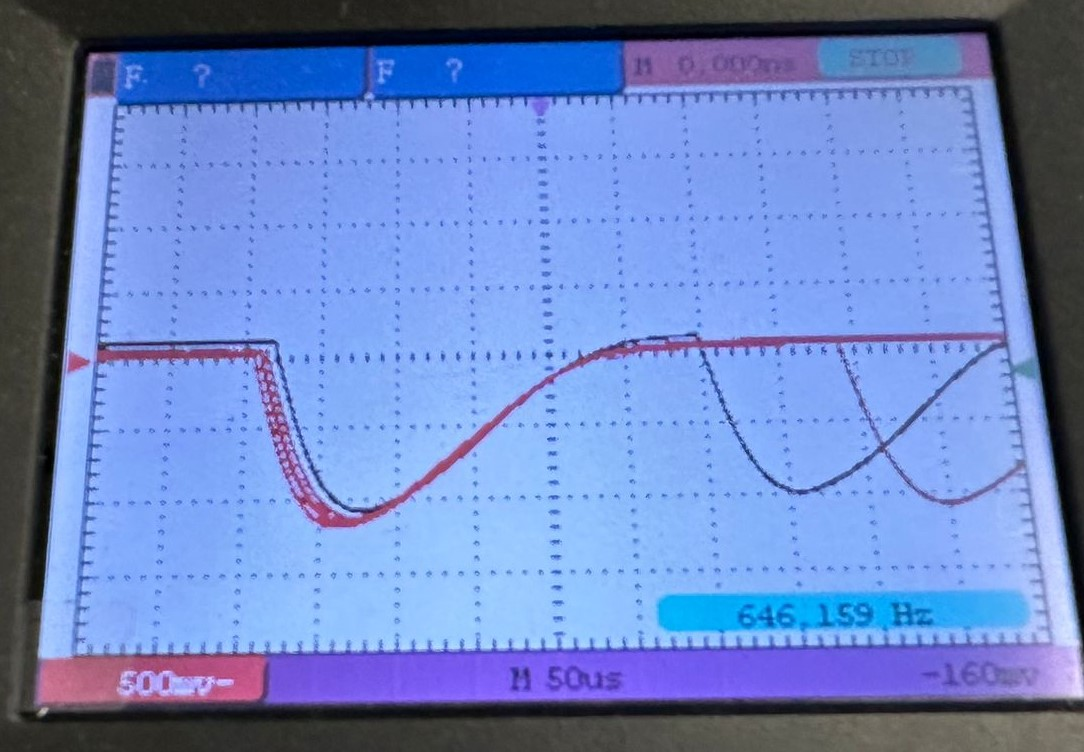
\includegraphics[width=0.5\linewidth]{data/totzeit.jpg}
	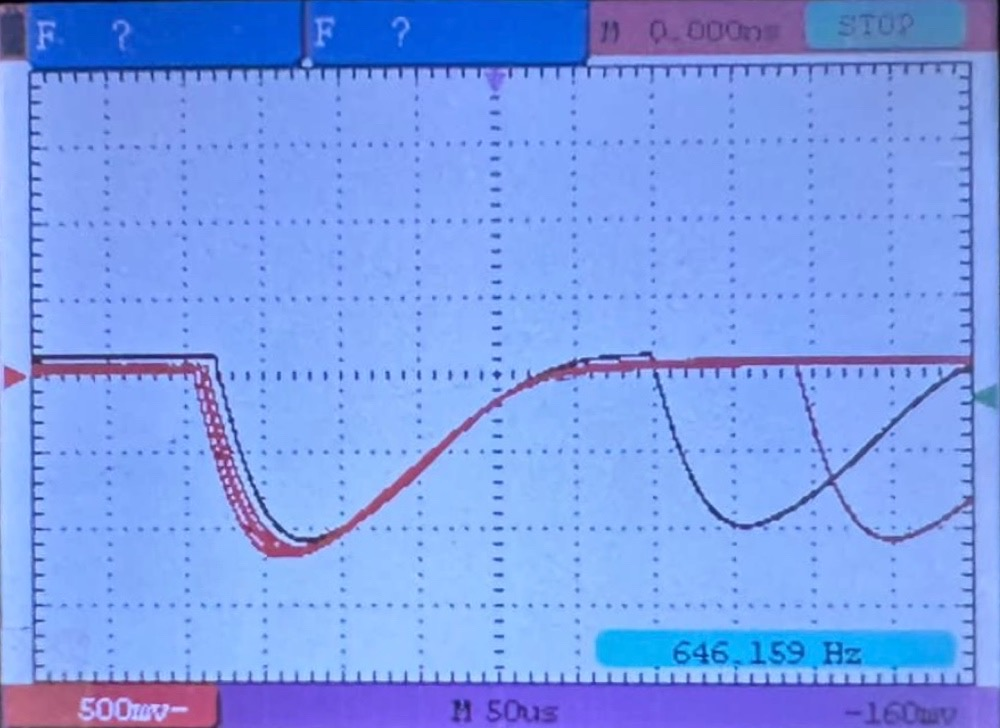
\includegraphics[width=0.5\linewidth]{content/grafik/zeit_1.jpg}
	\caption{Aufnahme des Osziloskops, an der die Totzeit und die Erholungszeit abgelesen werden kann.}
	\label{fig:totzeit}
\end{figure}
Es lässt sich der Wert 
\begin{equation*}
    \tau_{Osziloskop} = \left(3 \pm 0.2 \right) \cdot 50 \si{\micro\second} = \left(150 \pm  10\right) \si{\micro\second}
\end{equation*}
ablesen.
